\subsection{Tuning behaviour after Ozone switches}
\label{sec:switch}

This measurement was a preliminary measurement to perform the
transition from our pure Nitrogen Monoxide and synthetic air mixture
to unfiltered ambient air. The new challenge consists in the obvious
fact, that ambient air is not \ch{NO2} free. Thus if we add Ozone to
our sample air stream, we measure \ch{NO_x\, =\ NO + NO2}. In some
cases, e.\,g.\ during live vehicle measurements this is exactly what
we want (c.\,f.~Sec.~\ref{sec:vehicle}), however, in other cases we
would like to obtain the Nitrogen Monoxide and the Nitrogen Dioxide
concentrations separately. This can only be achieved indirectly. If we
have a single cavity, we can choose to measure \ch{NO2} and \ch{NO_x}
alternatingly by switching the Ozone stream off and on, we will denote
this as \emph{alternating measurement mode}. Doing that the technical
question arises how long we have to wait after triggering an Ozone
switch, before the equilibrium is reached and we can take our next
measurement.

As Section~\ref{sec:requirements} indicates, for a pathlength of
\SI{15}{\meter} we need about \SI{5.3}{\second} for the gas to be
completely exchanged. Taking the cavity volume itself into account a
\SI{30}{\second} purge time should well suffice for the exchange. As
will be seen during this section, there are other unpredicted effects,
which have a far longer decay time. These have to be further
understood before the alternating measurement mode should be used in a
productive system.

\subsubsection{Setup}
\label{sec:switch-setup}

This experiment was performed using the same setup as in
Section~\ref{sec:no} (c.\,f.\ Fig.~\ref{fig:no-setup} on
page~\pageref{fig:no-setup}). We fixed the flow of the \ch{NO}
calibration gas to $\Phi_{\ch{NO}} = \SI{0.01}{\liter\per\minute}$ and
kept all other flows as before. We set the cavity measurement script
to record 60 spectra sampled over 1000 scans each with an exposure
time of \SI{10}{\milli\second} then switch the Ozone stream on, record
60 spectra with the same characteristcs, switch the Ozone stream off
and repeat. With this setup we got a time resolution of
\SI{10}{\second}. In hindsight the sample size could have been
smaller to improve the time resolution. We performed the measurement
for both \SI{5}{\meter} and \SI{15}{\meter} reaction pathlength, due
to time constraints the measurement for \SI{10}{\meter} was shortened
to only collect 30 spectra. Thus we are missing some of the decay tail
in this case.

\subsubsection{Results}
\label{sec:switch-results}

Figure~\ref{fig:switch} contains the time series of the measured
\ch{NO2} concentration for a reaction pathlength of $l =
\SI{15}{\meter}$. The time series for the other two pathlengths were
similar in shape and are therefore omitted here. The flanks correspond
to the switch in the Ozone flow. There are severeal interesting
observations concerning this plot. First of all the increasing flanks
are very steep, which in this setting means, that the transition took
less than \SI{10}{\second}. The decreasing flanks take longer and
interestingly they do not reach \SI{0}{ppb}. This positive offset
could also be observed directly after the start of the measurement
(before any Ozone had been added to the 
sample air stream). The concentration rose to a level of
\SI{1.61(2)}{ppb}. One explanation for this is, that the calibration gas is
not \ch{NO2} free. This would raise the question why we did not
measure too much \ch{NO} in Section~\ref{sec:no}, since we actually
measured \ch{NO_x}. This question has three possible answers. First, the
\ch{NO} could have converted to \ch{NO2} over time in a ratio of
one to one. This would explain why we got the right results with the official
container concentration. Alternatively, the official concentration
might not have distinguished between \ch{NO} and \ch{NO2}, but might
have only been talking about a \ch{NO_x} concentration. This second
idea could be rejected after retrieving the calibration method, which
indeed distinguished between \ch{NO} and \ch{NO2}. The last possible
explanation is that the \ch{NO2} concentration might be negligible in
comparison to the amount of \ch{NO}, thus still allowing for the good
result in the previous chapter.

Accepting for the moment that we have a background \ch{NO2} signal, we
turn towards the question, why the decreasing flanks have the slowly
falling tail. In Figure~\ref{fig:switch-pl}, there are falling flanks for
different pathlenghts and we see that they all appear to have a
similar shape. They all seem to tend to the same equilibrium and the
decay time seems to grow with the pathlength. We suspect the reason
for this long tail to be a technical one. Between the Ozone valve and
the t-piece, connecting th Ozone stream to the sample air stream,
there is a \SI{14}{\centi\meter} tube filled with around
\SI{200}{ppm} Ozone. If this diffused into the sample line, this would
lead to further \ch{NO} conversion, although the Ozone stream had 
already been switched off. To investigate this hypothesis, we tried to fit
the decay using the following fit formula
\begin{align}
  f(t) \coloneqq c_0 + c_f \cdot\exp\left( -\frac{t}{\tau_f}\right) +
  c_s \cdot \exp\left(-\frac{t}{\tau_s}\right), \label{eq:switch-fit}
\end{align}
i.\,e.\ we suspect two overlaying decay processes. A fast one with a
decay time $\tau_f$ of less than $\SI{10}{\second}$ and a slower one
explaining the tail. Fitting this function we yielded the values
summarized in Table~\ref{tab:switch-coeff}. For the \SI{10}{\meter}
pathlength fit the offset concentration had to be fixed to
\SI{1.5}{ppb}, as the measured tail was too short for it to be
determined correctly.

\begin{table}[hbtp]
  \centering
  \begin{tabular}{rSSSSSS}
    \toprule
    {$l$}& {$\tau_f$} & {$\tau_s$} & {$c_0$} & {$c_f$} & {$c_s$} & {$V_{\ch{O3}}$}\\
    {\si{\meter}}& {\si{\second}} & {\si{\second}} & {\si{ppb}} & {\si{ppb}} &
                                                      {\si{ppb}} & {\si{10\tothe{-6}\milli\liter}}\\
    \midrule
    5 & 5.95 \pm 0.13 & 141 \pm 14 & 1.48 \pm 0.03 & 16.5 \pm 0.1 
                      & 1.46 \pm 0.07 & 6.9 \pm 0.8\\
    10 & 7.04 \pm 0.15 & 146 \pm 10 & 1.5 & 19.6 \pm 0.2
                       & 2.1 \pm 0.1 & 10.2 \pm 0.1\\
    15 & 10.15 \pm 0.12 & 193 \pm 12 & 1.52 \pm 0.03 & 21.0 \pm 0.1
                        & 2.36 \pm 0.06 & 15.2 \pm 0.2\\
    \bottomrule
  \end{tabular}
  \caption{Fit coefficients for the decay function
    (Eq.~\eqref{eq:switch-fit}) after an Ozone switch off. For the
    pathlength of $l= \SI{10}{\meter}$ the offset concentration was
    fixed to \SI{1.5}{ppb}. This was necessary as, due to the
    shortness of the measurement time, the tail was not long enough
    for the fit to determine the offset correctly. The last column
    contains the (partial) Volume of the Ozone participating in the
    reaction to form the long tail.}
  \label{tab:switch-coeff}
\end{table}
In any case the fits underline that we work with two time
scales. First a rather fast one, which is well described by the time
necessary for the gas to purge the system. And a second time scale in
the order of \SIrange{2.5}{3}{\minute}. To test our dead volume
hypothesis we want to use the fits to determine the amount of Ozone
necessary to explain the tail. We assume that the measured \ch{NO2}
signal above the offset, comes directly from the conversion of \ch{NO}
to \ch{NO2}. Looking at Reaction~\eqref{eq:no} on
page~\pageref{eq:no}, we see that this relation leads to a one to one
correspondence between the \ch{NO2} signal\footnote{always above the
offset} and the amount of Ozone enetering the sample air stream. To
determine the absolute amount, we integrate the slow falling part of
the fit function and use the constant flow of $\Phi =
\SI{2}{\liter\per\minute}$ to convert the result to the (partial)
volume of Ozone, i.\,e.
\begin{align*}
  V_{\ch{O3}} \coloneqq  c_s \cdot \tau_s \cdot \Phi.
\end{align*}
The result of this computation can be found in
Table~\ref{tab:switch-coeff}, too. We first notice the clear
pathlength dependence. This is already an indicator against our
hypothesis, as our dead volume is constant. Nevertheless, computing
the Ozone volume in the tube we get
\begin{align*}
  V_{\text{tube}} \approx \SI{3.52e-4}{\milli\liter(Ozone)}.
\end{align*}
This is even more evidence that the dead volume cannot be the sole
explanation. The total Ozone volume is about two orders of magnitude
too large. Even if we take into account that not the whole tube volume
contributes to the reaction (as the Ozone enters the sample air stream
via diffusion), we still have to explain the pathlength
dependence. Especially as it seems that the relation is highly linear,
one might suspect the reason to lie in the adsorption capacity of the
teflon tubes. This capacity would have to be researched more deeply
than we can provide at the current time, however, if the adsorption
plays an important role in the decay behaviour of the system, then we
have a further important restriction concerning the measurement
method. The alternating measurment mode would become impractical to
use, as the purge time would have to be in the order of magnitude of
multiple minutes. This is inacceptable for volatile environments as
for example urban areas.

\begin{figure}[htbp]
  \centering
  % GNUPLOT: LaTeX picture with Postscript
\begingroup
  \makeatletter
  \providecommand\color[2][]{%
    \GenericError{(gnuplot) \space\space\space\@spaces}{%
      Package color not loaded in conjunction with
      terminal option `colourtext'%
    }{See the gnuplot documentation for explanation.%
    }{Either use 'blacktext' in gnuplot or load the package
      color.sty in LaTeX.}%
    \renewcommand\color[2][]{}%
  }%
  \providecommand\includegraphics[2][]{%
    \GenericError{(gnuplot) \space\space\space\@spaces}{%
      Package graphicx or graphics not loaded%
    }{See the gnuplot documentation for explanation.%
    }{The gnuplot epslatex terminal needs graphicx.sty or graphics.sty.}%
    \renewcommand\includegraphics[2][]{}%
  }%
  \providecommand\rotatebox[2]{#2}%
  \@ifundefined{ifGPcolor}{%
    \newif\ifGPcolor
    \GPcolorfalse
  }{}%
  \@ifundefined{ifGPblacktext}{%
    \newif\ifGPblacktext
    \GPblacktexttrue
  }{}%
  % define a \g@addto@macro without @ in the name:
  \let\gplgaddtomacro\g@addto@macro
  % define empty templates for all commands taking text:
  \gdef\gplbacktext{}%
  \gdef\gplfronttext{}%
  \makeatother
  \ifGPblacktext
    % no textcolor at all
    \def\colorrgb#1{}%
    \def\colorgray#1{}%
  \else
    % gray or color?
    \ifGPcolor
      \def\colorrgb#1{\color[rgb]{#1}}%
      \def\colorgray#1{\color[gray]{#1}}%
      \expandafter\def\csname LTw\endcsname{\color{white}}%
      \expandafter\def\csname LTb\endcsname{\color{black}}%
      \expandafter\def\csname LTa\endcsname{\color{black}}%
      \expandafter\def\csname LT0\endcsname{\color[rgb]{1,0,0}}%
      \expandafter\def\csname LT1\endcsname{\color[rgb]{0,1,0}}%
      \expandafter\def\csname LT2\endcsname{\color[rgb]{0,0,1}}%
      \expandafter\def\csname LT3\endcsname{\color[rgb]{1,0,1}}%
      \expandafter\def\csname LT4\endcsname{\color[rgb]{0,1,1}}%
      \expandafter\def\csname LT5\endcsname{\color[rgb]{1,1,0}}%
      \expandafter\def\csname LT6\endcsname{\color[rgb]{0,0,0}}%
      \expandafter\def\csname LT7\endcsname{\color[rgb]{1,0.3,0}}%
      \expandafter\def\csname LT8\endcsname{\color[rgb]{0.5,0.5,0.5}}%
    \else
      % gray
      \def\colorrgb#1{\color{black}}%
      \def\colorgray#1{\color[gray]{#1}}%
      \expandafter\def\csname LTw\endcsname{\color{white}}%
      \expandafter\def\csname LTb\endcsname{\color{black}}%
      \expandafter\def\csname LTa\endcsname{\color{black}}%
      \expandafter\def\csname LT0\endcsname{\color{black}}%
      \expandafter\def\csname LT1\endcsname{\color{black}}%
      \expandafter\def\csname LT2\endcsname{\color{black}}%
      \expandafter\def\csname LT3\endcsname{\color{black}}%
      \expandafter\def\csname LT4\endcsname{\color{black}}%
      \expandafter\def\csname LT5\endcsname{\color{black}}%
      \expandafter\def\csname LT6\endcsname{\color{black}}%
      \expandafter\def\csname LT7\endcsname{\color{black}}%
      \expandafter\def\csname LT8\endcsname{\color{black}}%
    \fi
  \fi
    \setlength{\unitlength}{0.0500bp}%
    \ifx\gptboxheight\undefined%
      \newlength{\gptboxheight}%
      \newlength{\gptboxwidth}%
      \newsavebox{\gptboxtext}%
    \fi%
    \setlength{\fboxrule}{0.5pt}%
    \setlength{\fboxsep}{1pt}%
\begin{picture}(7200.00,5040.00)%
    \gplgaddtomacro\gplbacktext{%
      \csname LTb\endcsname%
      \put(682,704){\makebox(0,0)[r]{\strut{}$0$}}%
      \put(682,1383){\makebox(0,0)[r]{\strut{}$5$}}%
      \put(682,2061){\makebox(0,0)[r]{\strut{}$10$}}%
      \put(682,2740){\makebox(0,0)[r]{\strut{}$15$}}%
      \put(682,3418){\makebox(0,0)[r]{\strut{}$20$}}%
      \put(682,4097){\makebox(0,0)[r]{\strut{}$25$}}%
      \put(682,4775){\makebox(0,0)[r]{\strut{}$30$}}%
      \put(814,484){\makebox(0,0){\strut{}$0$}}%
      \put(1563,484){\makebox(0,0){\strut{}$500$}}%
      \put(2311,484){\makebox(0,0){\strut{}$1000$}}%
      \put(3060,484){\makebox(0,0){\strut{}$1500$}}%
      \put(3809,484){\makebox(0,0){\strut{}$2000$}}%
      \put(4557,484){\makebox(0,0){\strut{}$2500$}}%
      \put(5306,484){\makebox(0,0){\strut{}$3000$}}%
      \put(6054,484){\makebox(0,0){\strut{}$3500$}}%
      \put(6803,484){\makebox(0,0){\strut{}$4000$}}%
    }%
    \gplgaddtomacro\gplfronttext{%
      \csname LTb\endcsname%
      \put(176,2739){\rotatebox{-270}{\makebox(0,0){\strut{}Concentration [ppb]}}}%
      \put(3808,154){\makebox(0,0){\strut{}Time [s]}}%
    }%
    \gplbacktext
    \put(0,0){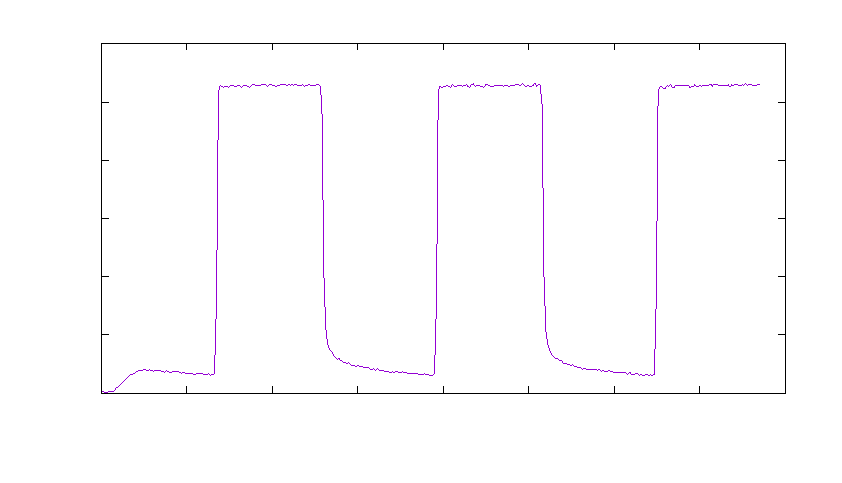
\includegraphics{../images/20160223_15_equil_fixI0_ts}}%
    \gplfronttext
  \end{picture}%
\endgroup

  \caption{Timeseries of the measured \ch{NO2} concentration while
    switching the Ozone stream on and off.}
  \label{fig:switch}
\end{figure}
If we want to persist on the alternating mode anyway and work with
shorter purge time, we would like to compensate
for the long tail. under the in thes experiment used laboratory
conditions, we know that we had
a constant supply of \ch{NO}, such that the behaviour of the falling
flank is solely determined by the changing Ozone concentration.
Assuming that the deca always follows Ecuation~\eqref{eq:switch-fit}
with the doefficients given in Table~\ref{tab:switch-coeff}, we can
compute the average additional \ch{NO2} signal due to the flank by

\begin{align}
  \bar c_s = \frac{c_s}{\Delta t} \int_{t_0}^{t_1}
  \exp\left(\frac{t}{\tau_s}\right)\d[t] \approx \SI{1.55(8)}{ppb},\label{eq:offset}
\end{align}
with $t_0 = \SI{30}{\second}$, $t_1 = \SI{60}{\second}$, $\Delta t =
t_1 - t_0$, where we already specialised to the later used setup of $l
= \SI{10}{\meter}$. We propose now to correct the measured \ch{NO2}
values by this offset. For this procedure to work, we would need th
edecay form to be mainly \ch{NO} independent. This assumption might be
true, as the bottle neck in Reaction~\eqref{eq:no} should be the
vanishing Ozone. However, to be sure, we would suggest to perform
further decay experiments at multiple \ch{NO} levels. This would lead
to the further advantage, that possible existing \ch{NO} dependencies
could possibly be extrapolated. This then could lead to a \ch{NO_x}
dependent offset correction in the evaluation procedure.
In the following we tested the limits of this rather crude
approximation. The results can be found in the next section.

\begin{figure}[htbp]
  \centering
  % GNUPLOT: LaTeX picture with Postscript
\begingroup
  \makeatletter
  \providecommand\color[2][]{%
    \GenericError{(gnuplot) \space\space\space\@spaces}{%
      Package color not loaded in conjunction with
      terminal option `colourtext'%
    }{See the gnuplot documentation for explanation.%
    }{Either use 'blacktext' in gnuplot or load the package
      color.sty in LaTeX.}%
    \renewcommand\color[2][]{}%
  }%
  \providecommand\includegraphics[2][]{%
    \GenericError{(gnuplot) \space\space\space\@spaces}{%
      Package graphicx or graphics not loaded%
    }{See the gnuplot documentation for explanation.%
    }{The gnuplot epslatex terminal needs graphicx.sty or graphics.sty.}%
    \renewcommand\includegraphics[2][]{}%
  }%
  \providecommand\rotatebox[2]{#2}%
  \@ifundefined{ifGPcolor}{%
    \newif\ifGPcolor
    \GPcolorfalse
  }{}%
  \@ifundefined{ifGPblacktext}{%
    \newif\ifGPblacktext
    \GPblacktexttrue
  }{}%
  % define a \g@addto@macro without @ in the name:
  \let\gplgaddtomacro\g@addto@macro
  % define empty templates for all commands taking text:
  \gdef\gplbacktext{}%
  \gdef\gplfronttext{}%
  \makeatother
  \ifGPblacktext
    % no textcolor at all
    \def\colorrgb#1{}%
    \def\colorgray#1{}%
  \else
    % gray or color?
    \ifGPcolor
      \def\colorrgb#1{\color[rgb]{#1}}%
      \def\colorgray#1{\color[gray]{#1}}%
      \expandafter\def\csname LTw\endcsname{\color{white}}%
      \expandafter\def\csname LTb\endcsname{\color{black}}%
      \expandafter\def\csname LTa\endcsname{\color{black}}%
      \expandafter\def\csname LT0\endcsname{\color[rgb]{1,0,0}}%
      \expandafter\def\csname LT1\endcsname{\color[rgb]{0,1,0}}%
      \expandafter\def\csname LT2\endcsname{\color[rgb]{0,0,1}}%
      \expandafter\def\csname LT3\endcsname{\color[rgb]{1,0,1}}%
      \expandafter\def\csname LT4\endcsname{\color[rgb]{0,1,1}}%
      \expandafter\def\csname LT5\endcsname{\color[rgb]{1,1,0}}%
      \expandafter\def\csname LT6\endcsname{\color[rgb]{0,0,0}}%
      \expandafter\def\csname LT7\endcsname{\color[rgb]{1,0.3,0}}%
      \expandafter\def\csname LT8\endcsname{\color[rgb]{0.5,0.5,0.5}}%
    \else
      % gray
      \def\colorrgb#1{\color{black}}%
      \def\colorgray#1{\color[gray]{#1}}%
      \expandafter\def\csname LTw\endcsname{\color{white}}%
      \expandafter\def\csname LTb\endcsname{\color{black}}%
      \expandafter\def\csname LTa\endcsname{\color{black}}%
      \expandafter\def\csname LT0\endcsname{\color{black}}%
      \expandafter\def\csname LT1\endcsname{\color{black}}%
      \expandafter\def\csname LT2\endcsname{\color{black}}%
      \expandafter\def\csname LT3\endcsname{\color{black}}%
      \expandafter\def\csname LT4\endcsname{\color{black}}%
      \expandafter\def\csname LT5\endcsname{\color{black}}%
      \expandafter\def\csname LT6\endcsname{\color{black}}%
      \expandafter\def\csname LT7\endcsname{\color{black}}%
      \expandafter\def\csname LT8\endcsname{\color{black}}%
    \fi
  \fi
    \setlength{\unitlength}{0.0500bp}%
    \ifx\gptboxheight\undefined%
      \newlength{\gptboxheight}%
      \newlength{\gptboxwidth}%
      \newsavebox{\gptboxtext}%
    \fi%
    \setlength{\fboxrule}{0.5pt}%
    \setlength{\fboxsep}{1pt}%
\begin{picture}(7200.00,5040.00)%
    \gplgaddtomacro\gplbacktext{%
      \csname LTb\endcsname%
      \put(682,704){\makebox(0,0)[r]{\strut{}$0$}}%
      \put(682,1518){\makebox(0,0)[r]{\strut{}$5$}}%
      \put(682,2332){\makebox(0,0)[r]{\strut{}$10$}}%
      \put(682,3147){\makebox(0,0)[r]{\strut{}$15$}}%
      \put(682,3961){\makebox(0,0)[r]{\strut{}$20$}}%
      \put(682,4775){\makebox(0,0)[r]{\strut{}$25$}}%
      \put(814,484){\makebox(0,0){\strut{}$0$}}%
      \put(1670,484){\makebox(0,0){\strut{}$100$}}%
      \put(2525,484){\makebox(0,0){\strut{}$200$}}%
      \put(3381,484){\makebox(0,0){\strut{}$300$}}%
      \put(4236,484){\makebox(0,0){\strut{}$400$}}%
      \put(5092,484){\makebox(0,0){\strut{}$500$}}%
      \put(5947,484){\makebox(0,0){\strut{}$600$}}%
      \put(6803,484){\makebox(0,0){\strut{}$700$}}%
    }%
    \gplgaddtomacro\gplfronttext{%
      \csname LTb\endcsname%
      \put(176,2739){\rotatebox{-270}{\makebox(0,0){\strut{}Concentration [ppb]}}}%
      \put(3808,154){\makebox(0,0){\strut{}Time [s]}}%
      \csname LTb\endcsname%
      \put(5816,4602){\makebox(0,0)[r]{\strut{}$\SI{05}{\meter}$}}%
      \csname LTb\endcsname%
      \put(5816,4382){\makebox(0,0)[r]{\strut{}$\SI{10}{\meter}$}}%
      \csname LTb\endcsname%
      \put(5816,4162){\makebox(0,0)[r]{\strut{}$\SI{15}{\meter}$}}%
    }%
    \gplbacktext
    \put(0,0){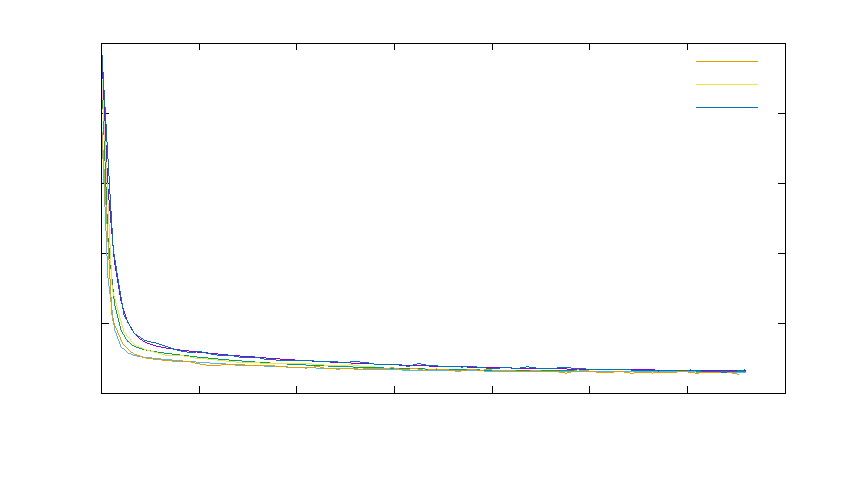
\includegraphics{../images/20160223_equil_fixI0_fall_fit}}%
    \gplfronttext
  \end{picture}%
\endgroup

  \caption{The behaviour of the falling flanks depending on the
    reaction pathlength}
  \label{fig:switch-pl}
\end{figure}


%%% Local Variables:
%%% mode: latex
%%% TeX-master: "../Bachelor"
%%% End:
